% ============================================================
% S20 — Modèle de production & apprentissages
% ============================================================
\begin{frame}{Produire en équipe, et ce que j'y ai appris}
  \framesubtitle{Un cadre agile adapté à la recherche}
  \begin{columns}[T,onlytextwidth]
    \column{0.52\textwidth}
      \begin{itemize}
        \item \textbf{Scrum} : sprints d'une semaine, backlog Kanban, Jira
        \item Scrum Master \textbf{tournant}, poker planning, dailies
        \item Comités hebdomadaires $=$ sprint reviews scientifiques
        \item \textbf{JdS} : restitution devant les collaborateurs Aubay + article de blog interne
      \end{itemize}
      \vspace{0.15cm}
      \begin{block}{Évaluation entreprise}
        \small Mention « \textbf{Excellente} » (7 juillet 2026)
      \end{block}
    \column{0.44\textwidth}
      \centering
      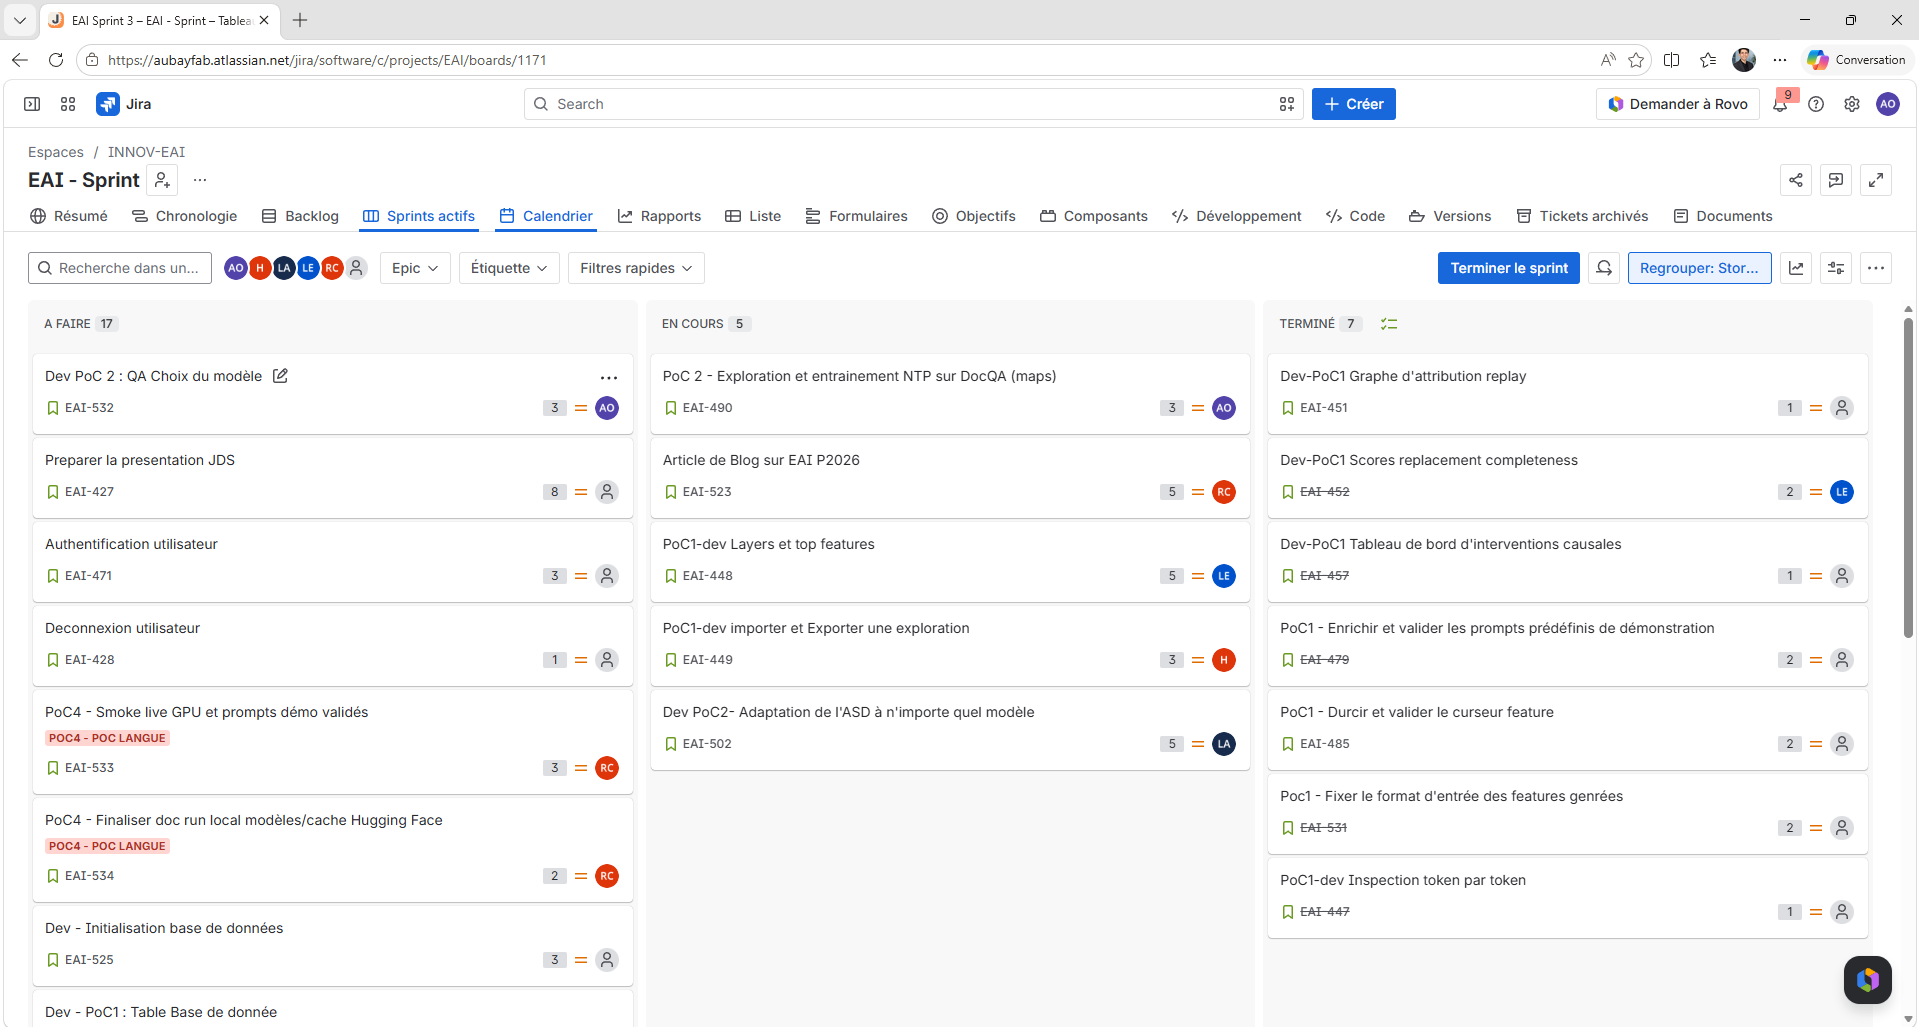
\includegraphics[width=\linewidth,height=0.42\textheight,keepaspectratio]{media/jira_sprint.png}
      \vspace{0.2cm}
      \AubayFocusPanel{Mon axe de progrès (assumé)}{La \textbf{synchronisation} : sur un travail en binôme, j'ai parfois avancé trop vite seul. Les dailies et le poker planning m'ont appris à exposer mes choix \textbf{avant} de les coder.}
  \end{columns}
  \AubayTraceRef{A.6.1}
\end{frame}
